\chapter{Python op de Pi}

\section{Introductie linux terminal}\index{Introductie linux terminal}

\section{Editor}\index{Editor}
Net als bij je laptop is het ook op de \textit{Pi} handiger om een \textit{IDE} te gebruiken. Als het goed is staat \textit{Thonny} standaard geïnstalleerd, maar ook hier mag je alles gebruiken wat je zelf prettig vindt. Tijdens de lessen wordt zoals eerder vermeld met Thonny gewerkt. \newline

Mocht \textit{Thonny} of je favoriete editor nog niet geïnstalleerd zijn, is dit een mooi moment om te kijken dat eigenlijk gaat onder \textit{Linux}. Je kunt hiervoor de grafische \textit{Add/Remove Software}-tool voor gebruiken:
\begin{figure}[h!]
\centering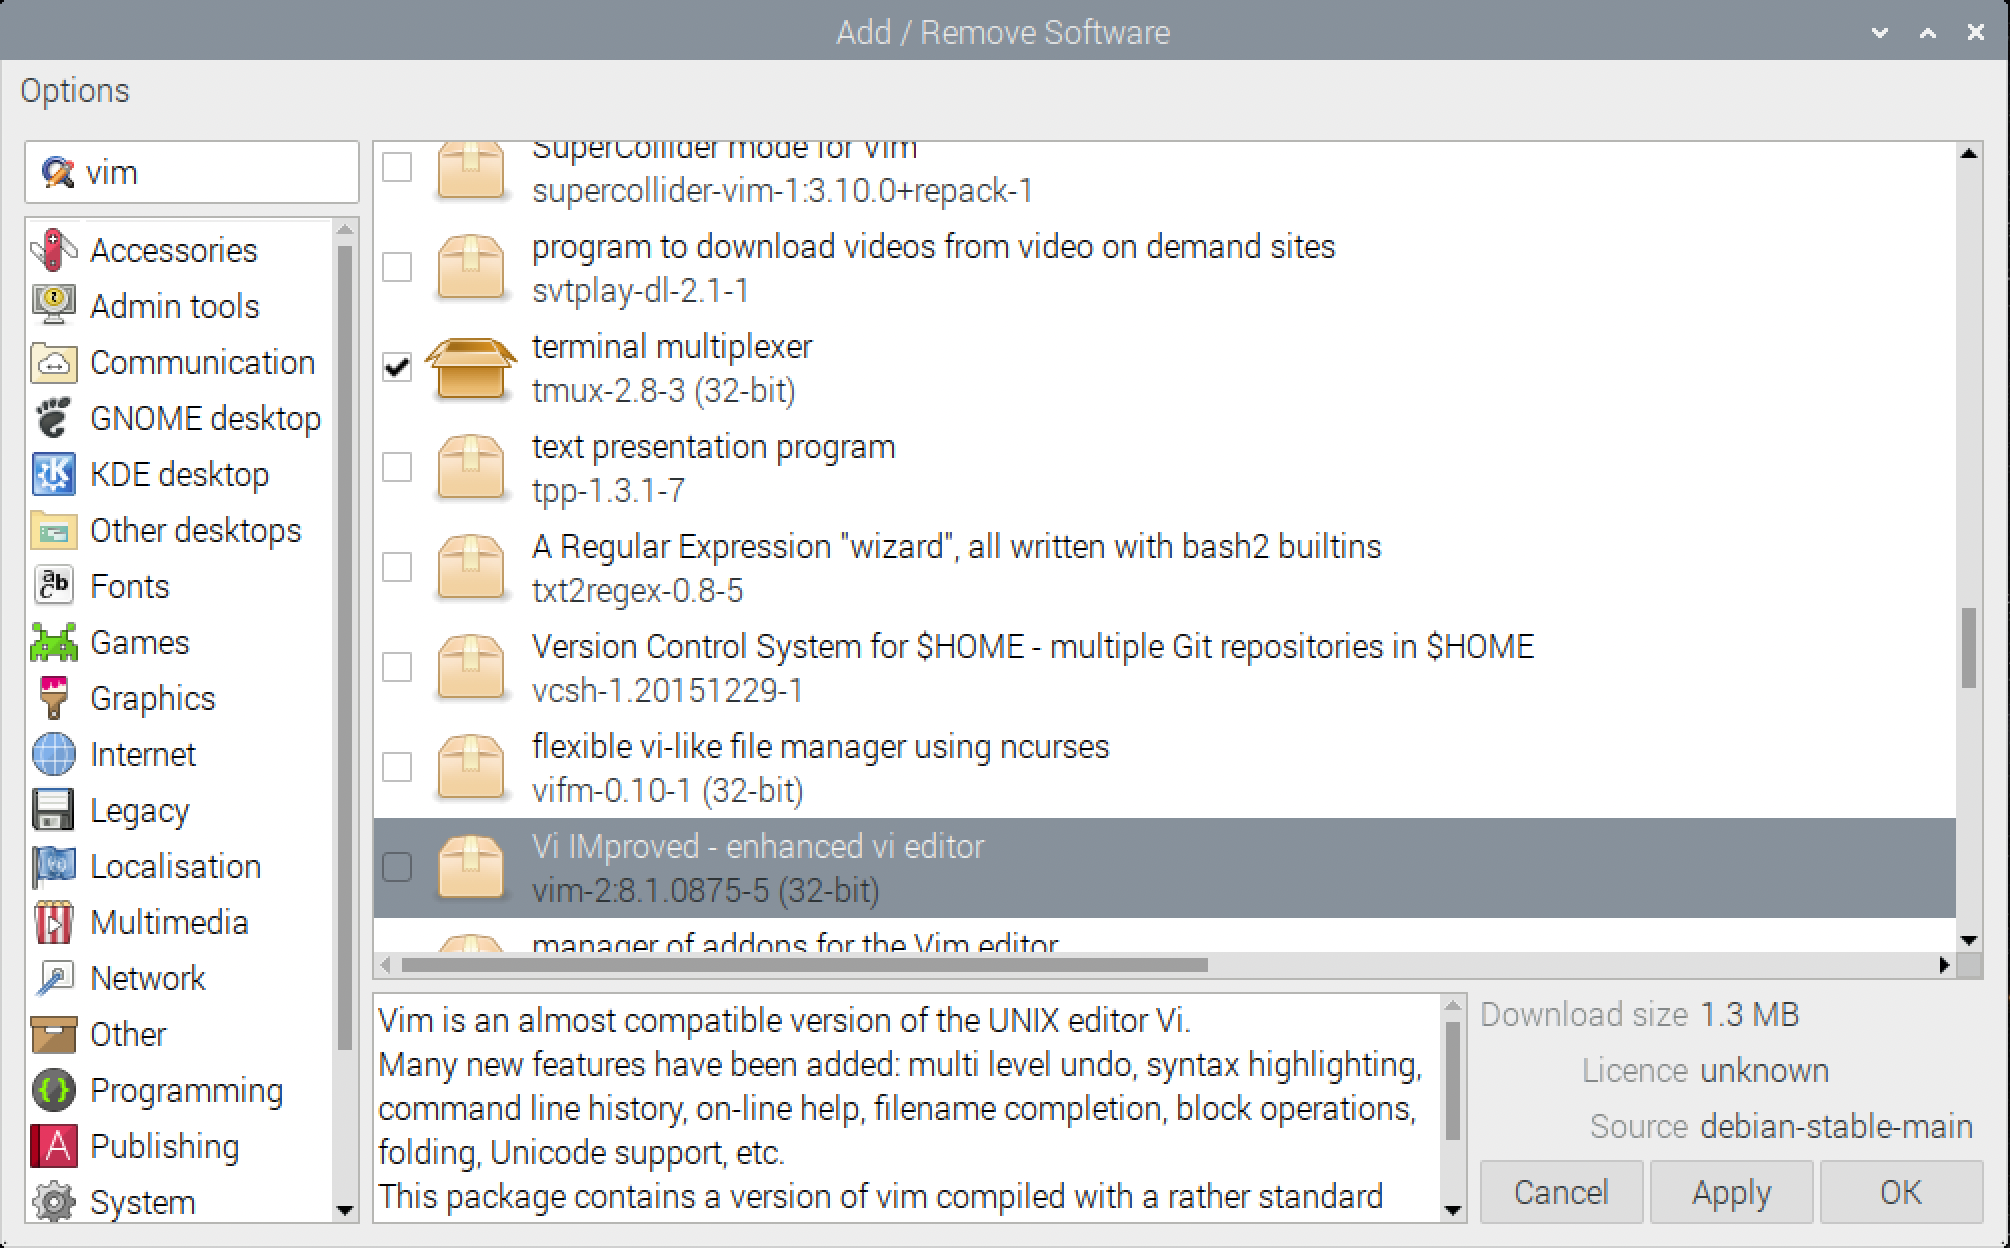
\includegraphics[scale=0.35]{Pictures/chapter05/add_remove_software.png}
\caption{\textit{Add/Remove Software} tool}
\label{fig:addremovesoftware} % Unique label used for referencing the figure in-text
%\addcontentsline{toc}{figure}{Figure \ref{fig:webserver}} % Uncomment to add the figure to the table of contents
\end{figure}

\begin{remark}
Een beetje hacker doet dit vaak via de \textit{Terminal}. Ook omdat de \textit{Pi} niet altijd aangesloten is op een scherm, is het ook handig om te weten hoe dit werkt. Allereerst zorg je ervoor dat alle lijsten met software die je kunt installeren up-to-date is:
\begin{lstlisting}[language=bash]
sudo apt-get update
\end{lstlisting}

Daarna installeer je het programma in kwestie:
\begin{lstlisting}[language=bash]
sudo apt-get install thonny
\end{lstlisting}
Als dit klaar is, is je vers geïnstalleerde programma te vinden in het \textit{Pi-menu} linksboven.
\end{remark}

\section{Pi header}\index{Pi header}

\section{GPIO}\index{GPIO}

\section{Loops}\index{Loops}
Als we bepaalde onderdelen van onze code vaker uit willen voeren, kunnen we dat doen aan de hand van \textit{loops}. In \textit{C} hadden we al kennisgemaakt met de \pyth{for}-loop. Deze zit gelukkig ook in \textit{Python}, maar werkt wel een beetje anders. We gebruiken deze vaak in combinatie met de funtie \pyth{range()}:
\begin{python}
for x in range(0, 10, 1):
	print(x)
\end{python}
In het bovenstaande voorbeeld roepen we de functie \pyth{range()} aan met 3 argumenten. De eerste geeft het startgetal voor $x$ aan, de tweede bij welke waarde van $x$ de loop moet stoppen, en de derde en laatste met welke hoeveel we $x$ we moeten verhogen bij elke nieuwe iteratie. Dit voorbeeld print dus de getallen $0$ t/m $9$ op het scherm:
\begin{python}
0
1
2
3
4
5
6
7
8
9
\end{python}

\begin{remark}
De functie \pyth{range()} kun je op $3$ verschillende manieren aanroepen:
\begin{enumerate}
\item[-] \pyth{range(stop)}: Met enkel $1$ argument, de stop waarde. $start=0, step=1$.
\item[-] \pyth{range(start, stop)}: Met $2$ argumenten, voor start en stop. $step=1$.
\item[-] \pyth{range(start, stop, stap)}: En $3$, zoals in het voorbeeld.
\end{enumerate}
In het bovenstaande stukje voorbeeldcode kan dus \pyth{range(0, 10, 1)} worden vervangen door \pyth{range(10)}, want die levert dezelfde functionaliteit.
\end{remark}

Als tweede voorbeeld een loop die van $2$ t/m $25$ loopt, met stapjes van $3$:
\begin{python}
for x in range(2, 25, 3):
	print(x)
\end{python}
Dit print het volgende uit: $2, 5, 8, 11, 14, 17, 20, 23$. De \pyth{for}-loop stopt na $23$, omdat $23+3 = 26$, wat hoger is dan $25$, de stop waarde. \newline\newline

Naast de \pyth{for}-loop, bestaat er ook de \pyth{while}-loop. Deze zit ook in \textit{C}, maar hebben we destijds niet gebruikt. Wellicht is het handig om te weten dat hij bestaat, en te snappen hoe je 'm gebruikt:
\begin{python}
i = 1
while i < 6:
	print(i)
	i += 1
\end{python}
In het bovenstaand voorbeeld wordt de code in de \pyth{while}-loop uitgevoerd \textit{zolang} de conditie \pyth{i < 6} gelijk is aan \pyth{True}. We beginnen met \pyth{i = 1}, en tellen er elke keer \pyth{1} bij op, waardoor de uitvoer van het programma $1$ t/m $5$ is. \par

Met een \pyth{while}-loop is ook vrij makkelijk een oneindige loop te maken, vergelijkbaar met de \textit{loop()}-functie bij de \textit{Arduino}:
\begin{python}
while True:
	print('en door..')
\end{python}

\begin{remark}
Het is bij zo'n loop wel handig om te weten hoe je 'm weer stopt. Want in de meeste gevallen maak je 'm per ongeluk. Bij een \textit{IDE} heb je naast een run knopt (groen driehoekje), vaak ook een stop knop (rood vierkantje). In de terminal kun je de toetscombinatie \text{Ctrl+C} gebruiken. 
\end{remark}

\newpage

\section{Huiswerkopdrachten}\index{Huiswerkopdrachten}
\begin{exercise}
Schrijf een programma waarin je met een \pyth{while}-loop de eerste $10$ getallen van de tafel van $5$ print.
\end{exercise}

\begin{exercise}
Schrijf een programma waarin je de gebruiker vraagt om een getal, en geef daarna de eerste $10$ getallen van de tafel voor dat getal. Gebruik hiervoor een \pyth{for}-loop.
\end{exercise}

\begin{exercise}
Schrijf een programma die de getallen van $-10$ t/m $-1$ op scherm print. Gebruik hiervoor alleen de \pyth{range()}-functie in de \pyth{for}-loop (en natuurlijk een \pyth{print()} ;) ).
\end{exercise}

\begin{exercise}\label{exc5:exc4}
Vraag aan de gebruiker een getal $l$, en print daarna een rij van sterretjes. Dus bij $l=7$, geeft het de volgende output:
\begin{python}
*******
\end{python}
\textbf{TIP:} Als je niet wilt dat een \pyth{print}-functie elke keer een nieuwe regel begint, kun je dit veranderen door het \textit{end}-argument te gebruiken: \pyth{print('*', end='')}. 
\end{exercise}


\begin{exercise}
Breid Vraag \ref{exc4:exc1} uit. Vraag aan de gebruiker nu $2$ getallen: $h$ en $l$. Print daarna een vierkant van sterretjes ter grootte van $h \times l$. Dus bij $h=3$ en $l=5$, geeft het de volgende output:
\begin{python}
*****
*****
*****
\end{python}
\textbf{TIP:} Je kunt loops in loops zetten. 
\end{exercise}

\begin{exercise}
$\\$
\end{exercise}

\begin{exercise}
$\\$
\end{exercise}

\begin{exercise}
$\\$
\end{exercise}

\begin{exercise}
$\\$
\end{exercise}

